\section{AES}
Nel 1998 esce il bando per ricercare un nuovo algoritmo per soppiantare il DES ed il 3DES.
Ci furono 21 proposte che dovevano tenere conto di
\begin{itemize}
    \item sicurezza: resistere a tutti gli attacchi noti
    \item costo di realizzazione: doveva essere facile implementarlo sia in software che in hardware
    \item caratteristiche algoritmiche: portabile su diverse macchine, usabile con chiavi di diversa lunghezza
    \item libero da brevetti in quanto il nuovo standard doveva divenire libero da utilizzare
\end{itemize}

Nell'Ottobre del 2000 si sceglie l'AES e nel 2001 diventa lo standard.
E' un algoritmo che ancora oggi continua a conservare tutti i bit di sicurezza.
Gli altri 4 cifrari arrivati alla fine erano:
\begin{itemize}
    \item MARS (IBM)
    \item RCG (RSA)
    \item Rijndael (Proton word int + Università di Leuven, Belgio)
    \item SERPENT (Università di Israele, UK, USA)
    \item TWOFISH (Berkeley, Princeton)
\end{itemize}
Rijndael vince il bando e diventa AES con qualche modifica.

Permette chiavi di 128, 192, 256 bit, ma noi vedremo la versione a 128 bit.
Si usa su blocchi anch'essi di 128 bit. Funziona per fasi:
\begin{itemize}
    \item 10 fasi $\xrightarrow{}$ 128 bit
    \item 12 fasi $\xrightarrow{}$ 192 bit
    \item 14 fasi $\xrightarrow{}$ 256 bit
\end{itemize}

\subsection{Selezione delle sottochiavi di fase}
Si parte da 128 bit di chiave posizionati in una matrice $4 \times 4$ byte per colonna:

$$
K = 
    \begin{bmatrix}
        K[0] & K[4] & K[8] & K[12] \\
        K[1] & K[5] & K[9] & K[13] \\
        K[2] & K[6] & K[10] & K[14] \\
        K[3] & K[7] & K[11] & K[15]
    \end{bmatrix}
$$

Prese le colonne in ordine da sinistra verso destra abbiamo: 
$$W(0), W(1), W(2), W(3)$$
Costruiamo quindi $W(i)$ che è una sequenza di byte che usiamo per generale le sottochiavi di fase.
Per ogni $t \geq 4$:
\begin{equation}
    W(t) = 
    \begin{cases}
        W(t-1) \oplus W(t-4) \text{ se t non è multiplo di 4} \\
        T(W(t-1)) \oplus W(t-4) \text{ se t è multiplo di 4}
    \end{cases}
\end{equation}

T è una funzione non lineare applicata tramite una S-box.
La chiave dell'$i$-esima fase è quindi composta da:
$W(4 \cdot i), W(4 \cdot i + 1), W(4 \cdot i + 2), W(4 \cdot i + 3),$

\subsection{Preparazione}
La cifratura si fa per blocchi (di 128 bit in questo caso).
Si creano i blocchi caricandoli \emph{per colonna} in una matrice $4 \times 4$ byte:
$$
B = 
    \begin{bmatrix}
        b_{00} & b_{01} & b_{02} & b_{03} \\
        b_{10} & b_{11} & b_{12} & b_{13} \\
        b_{20} & b_{21} & b_{22} & b_{23} \\
        b_{30} & b_{31} & b_{32} & b_{33}
    \end{bmatrix}
    b_{ij} \in \{0, 1\}^{8}
$$

Si applica una prima trasformazione applicando la chiave:
$$ B \oplus K $$

\subsection{Fasi}
Dopodiché si inizia con le fasi, ognuna di esse composta da 4 operazioni:
\begin{itemize}
    \item \emph{substitution bytes}
    \item \emph{shift rows}
    \item \emph{mix columns}
    \item \emph{add round key}
\end{itemize}
Le prime 3 operazioni applicano: non linearità, diffusione e confusione.
L'ultima fase aggiunge la chiave.

Nell'ultima fase \emph{non} si applica la mix columns. Alla fine delle iterazioni si ottiene il crittogramma.
La S-Box dell'AES è sempre usata in forma di tabella di verità, ma a differenza di quella del DES si conosce la funzione che la genera!

\subsection{Substitution bytes}
Ogni byte viene trasformato usando la S-Box:
$$ b_{ij} \xrightarrow{} S-Box(b_{ij}) $$

Questa S-Box si compone di una matrice $16 \times 16$ di interi $\in [0, 255]$ e contiene una permutazione dei numeri di questo intervallo.
L'accesso alla S-Box viene fatto suddividendo il byte $b_{ij}$ in due blocchi da 4 bit l'uno:
$$ b_{ij} = b_{1}b_{2}b_{3}b_{4} \mid b_{5}b_{6}b_{7}b_{8} $$
i primi 4 bit formano il numero di \emph{riga}, gli ultimi 4 bit formano il numero di colonna.

La relazione implementata dalla S-Box è:
$$ x \xrightarrow{} x^{-1} + c $$
questo inverso è l'inverso moltiplicativo in $GF(2^{8})$ con l'aggiunta di una componente lineare.
In questo insieme la somma viene eseguita tramite lo XOR (somma modulo 8), mentre la moltiplicazione è eseguita $\mod 2^{8}$.
Nella pratica ogni byte può essere visto come un polinomio, facendo la moltiplicazione si fa il prodotto tra polinomi ma in modulo, quindi si tagliano via i gradi oltre al settimo.
NB: GF: Galois Field - campi finiti di Galois

Questa S-Box ha una bassissima correlazione tra i bit di ingresso e di uscita.
Inoltre essendo usata sia per la chiave che per la matrice del messaggio si ha una maggiore sicurezza

\subsection{Shift rows}
Si usa per spargere il messaggio.
Lascia invariata la prima riga, shifta a sx di 1, 2, 3 le altre righe, rispettivamente.

$$
    \begin{bmatrix}
        b_{00} & b_{01} & b_{02} & b_{03} \\
        b_{10} & b_{11} & b_{12} & b_{13} \\
        b_{20} & b_{21} & b_{22} & b_{23} \\
        b_{30} & b_{31} & b_{32} & b_{33}
    \end{bmatrix}
\xrightarrow{}
    \begin{bmatrix}
        b_{00} & b_{01} & b_{02} & b_{03} \\
        b_{11} & b_{12} & b_{13} & b_{10} \\
        b_{22} & b_{23} & b_{20} & b_{21} \\
        b_{33} & b_{30} & b_{31} & b_{32}
    \end{bmatrix}
$$
Ho quindi diffuso i byte di ogni colonna su tutte le altre.

\subsection{Mix columns}
Si mixano le colonne attraverso una moltiplicazione per matrice.
M matrice $4 \times 4$ byte, per ogni colonna:
$$
    B_{j} \xrightarrow{} M \cdot B_{j}
$$
Anche qui si lavora in GF($2^8$). Questo porta ogni elemento della colonna ad essere dipendente da tutti i byte della colonna.

\subsection{Add round key}
$$
    b_{ij} \xrightarrow{} b_{ij} \oplus K_{ij} \text{ chiave della sottofase}
$$
NB: si noti che shift rows e mix columns arrivano alla massima diffusione già al secondo round in quanto ogni byte è dipendente da tutti gli altri del messaggio.

NB: i 128 bit sono tutti bit di sicurezza ancora oggi!

Esistono attacchi che rendono vulnerabile il cifrario se usato con 6 round, lo standard tuttavia ne vuole 10 quindi fino ad ora non abbiamo nessun problema.

E' vulnerabile ad attacchi di tipo \emph{side-channel} ma questi attacchi sono indipendenti dal sistema.

\subsection{Cifratura a blocchi}
Sia il DES che l'AES cifrano il plaintext a blocchi, AES ad esempio divide in blocchi grandi quanto la chiave e poi si cripta.
Il problema di ciò è che blocchi uguali vengono cifrati in blocchi uguali, questo può dare molte informazioni.
Per risolvere questo problema si cerca di inserire una dipendenza tra il blocco $i$-esimo e quelli che vengono prima.
Nell'AES si prende $m$ e lo si divide in blocchi da 128 bit:
$$ m = m_{1}m_{2}\_m_{i}\_m_{e} $$
se $\mid m_e \mid < 128$ allora si aggiunge $10...0$ fino ad arrivare a 128, se invece $\mid m_e \mid = 128$ si inserisce un intero blocco $10...0$ in modo da avere sempre questo terminatore.
Successivamente si sceglie una $c_0$ random che può anche essere trasmessa in pari a si attua questo schema:
\begin{figure}[H]
    \centering
    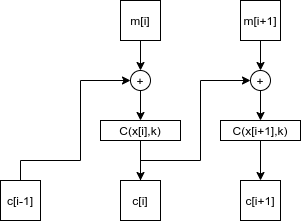
\includegraphics[width = 200pt]{CBC.png}
\end{figure}

$$
    x_{i} = m_{i} \oplus c_{i-1}
$$
$$
    c_{i} = C(m_{i} \oplus c_{i-1}, K)
$$
questa modalità è detta \emph{CBC: Cipher Block Chaining}.
La decifrazione invece si esegue in questo modo:
\begin{figure}[H]
    \centering
    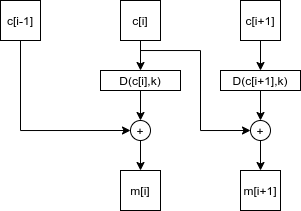
\includegraphics[width = 200pt]{CBC_2.png}
\end{figure}

$$
    m_i = D(c_i, K) \oplus c_{i-1}
$$

NB: mentre la cifratura va eseguita necessariamente sequenzialmente la decifratura si può eseguire in parallelo.
Inoltre se invio il testo cifrato e ci sono errori risolta in un errata decifrazione solo del blocco $i$ e $i+1$ mentre gli altri continuano ad essere decriptati correttamente.

\subsection{Altri cifrari simmetrici}
\begin{itemize}
    \item \emph{Ron's Code 5} (RC5): simile al DES, ma migliorato.
    Blocchi da 64 bit e chiavi di $c \cdot 32$ bit, $r$ fasi (consigliate 16). $r$ e $c$ scelti a piacere. Usa shift ciclico, XOR, addizione $\mod 2^{32}$. Semplice da realizzare e sicuro
    \item \emph{International Data Encryption Algorithm} (IDEA): chiave a 128 bit, usa shift ciclico, XOR, moltiplicazione $\mod (2^{16} + 1)$ ed addizione $\mod 2^{16}$. Più semplice e sicuro del DES
\end{itemize}